% \part{First Part}
\chapter{Introduction}
\section{Background}
\subsection{Related Work}
\subsubsection{Methodology}
\paragraph{Data Collection}
\subparagraph{Sampling}
Place your image in chapters/images folder. Refer \ref{fig:waterfall}
\begin{figure}
	\centering
	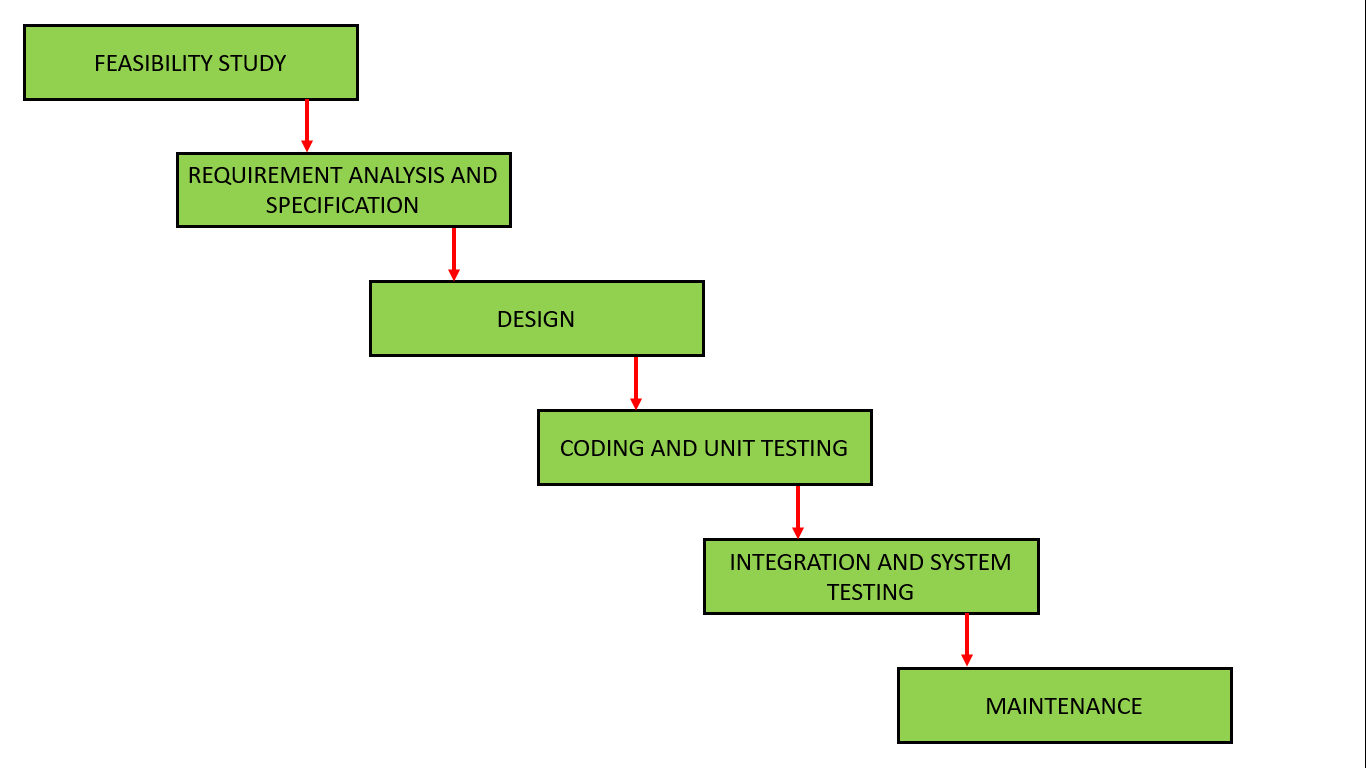
\includegraphics[scale=0.15]{chapters/images/waterfall.png}
	\caption{Various stages involved in the waterfall model}
	\label{fig:waterfall}
\end{figure}

\section{Code snippets}
Place your code snippets in codes folder. Refer \ref{fig:sample_code} 
\begin{figure}

	\begin{lstlisting}
		#include <iostream>
		
		int main() {
			std::cout << "Hello, World!" << std::endl;
			return 0;
		}
	\end{lstlisting}

	\caption{Sample function.}
	\label{fig:sample_code}
\end{figure}


\section{Tables}
\begin{table}
	\centering
	\begin{tabular}{l|l}
		A & B \\
		\hline 
		1 & 2 
	\end{tabular}
	\caption{Sample table}
	\label{tab:highlights}
\end{table}

\section{Abbreviations}
Abbreviation

\section{Footnotes}
You can add footnotes \footnote{Sample footnote}
You can also add another \footnote{Second Footnote}

\section{References}
Add BibTeX format bibliography entries in bib.bib and cite anywhere like this; \cite{cite1}. The another systematic approach for this is as follows as the order of the system grows the mechnical system is difficult to handle. \cite{cite2}. The another line The another systematic approach for this is as follows as the order of the system grows the mechnical system is difficult to handle. \cite{cite3} . The another line \cite{cite4}. The next line \cite{cite5}. This is fifth citation of the text. \cite{cite1,cite4}. The citation of first and fourth references.



The another level \footnote{foot3} of text is here.



